\documentclass[]{tufte-book}

% ams
\usepackage{amssymb,amsmath}

\usepackage{ifxetex,ifluatex}
\usepackage{fixltx2e} % provides \textsubscript
\ifnum 0\ifxetex 1\fi\ifluatex 1\fi=0 % if pdftex
  \usepackage[T1]{fontenc}
  \usepackage[utf8]{inputenc}
\else % if luatex or xelatex
  \makeatletter
  \@ifpackageloaded{fontspec}{}{\usepackage{fontspec}}
  \makeatother
  \defaultfontfeatures{Ligatures=TeX,Scale=MatchLowercase}
  \makeatletter
  \@ifpackageloaded{soul}{
     \renewcommand\allcapsspacing[1]{{\addfontfeature{LetterSpace=15}#1}}
     \renewcommand\smallcapsspacing[1]{{\addfontfeature{LetterSpace=10}#1}}
   }{}
  \makeatother

\fi

% graphix
\usepackage{graphicx}
\setkeys{Gin}{width=\linewidth,totalheight=\textheight,keepaspectratio}

% booktabs
\usepackage{booktabs}

% url
\usepackage{url}

% hyperref
\usepackage{hyperref}

% units.
\usepackage{units}


\setcounter{secnumdepth}{-1}

% citations
\usepackage{natbib}
\bibliographystyle{plainnat}


% pandoc syntax highlighting

% table with pandoc
\usepackage{longtable,booktabs,array}
\usepackage{calc} % for calculating minipage widths
% Correct order of tables after \paragraph or \subparagraph
\usepackage{etoolbox}
\makeatletter
\patchcmd\longtable{\par}{\if@noskipsec\mbox{}\fi\par}{}{}
\makeatother
% Allow footnotes in longtable head/foot
\IfFileExists{footnotehyper.sty}{\usepackage{footnotehyper}}{\usepackage{footnote}}
\makesavenoteenv{longtable}

% multiplecol
\usepackage{multicol}

% strikeout
\usepackage[normalem]{ulem}

% morefloats
\usepackage{morefloats}


% tightlist macro required by pandoc >= 1.14
\providecommand{\tightlist}{%
  \setlength{\itemsep}{0pt}\setlength{\parskip}{0pt}}

% title / author / date
\title[Selection Criteria]{SIVOCS Interview Candidates}
\date{2022-07-22}


\begin{document}

\maketitle




\hypertarget{selection-steps}{%
\chapter{Selection Steps}\label{selection-steps}}

The selection of \textasciitilde60 candidates for the interview process
has been carried out with a clustering approach. Each of the clusters
has been arranged with consideration of some of the most central
variables in identifying Social Innovation (SI) which have been
determined previously in the study.

The distribution of some of the important variables as well as their
correlations with each other can be seen in the Figure @ref(fig:corr).

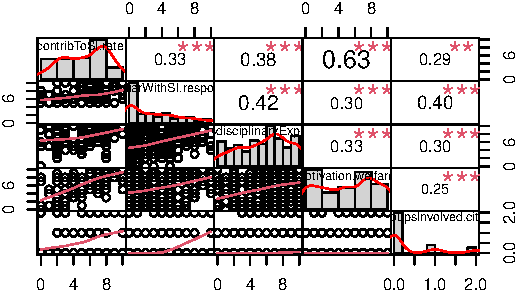
\includegraphics{03_SIVOCS_int-cand_files/figure-latex/corr-1}

\hypertarget{step-1-contribution-to-si-self-assessment}{%
\section{Step 1: Contribution to SI
(self-assessment)}\label{step-1-contribution-to-si-self-assessment}}

The first criterion was selected to find easily identifiable (obvious)
SI-related projects. The selection has relied on the self-assessment of
the participants about the contribution their specific project made to
the SI.

The selected 34 (28m \textbar{} 6f) participants are lying between the
3rd quantile (8) and maximum value (10) on the scale of the variable
\emph{contribution to SI}, the distribution of the variable can be seen
in Figure@ref(fig:step1).

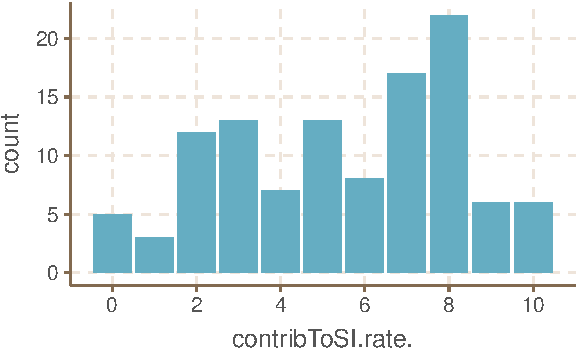
\includegraphics{03_SIVOCS_int-cand_files/figure-latex/step1-1}

\hypertarget{step-2-experience-with-transdisciplinarity-contribution-to-si-sci.-disciplines}{%
\section{Step 2: Experience with transdisciplinarity, contribution to
SI, sci.
disciplines}\label{step-2-experience-with-transdisciplinarity-contribution-to-si-sci.-disciplines}}

After excluding the selected participants in the previous step the
participants who have placed themselves between the 3rd quantile (8) and
maximum value (10) on the variable \emph{experience with
transdisciplinarity} selected for step 2. The first examination included
fitting a linear regression model to investigate the relation between
\emph{experience with transdisciplinarity} and \emph{contribution to
SI}. A visualisation regarding this model can be seen in Figure
@ref(fig:td\_si\_lm)\footnote{Caution: The figure includes the whole
  sample, not just the reduced sample after excluding the chosen
  participants in step 1.}.

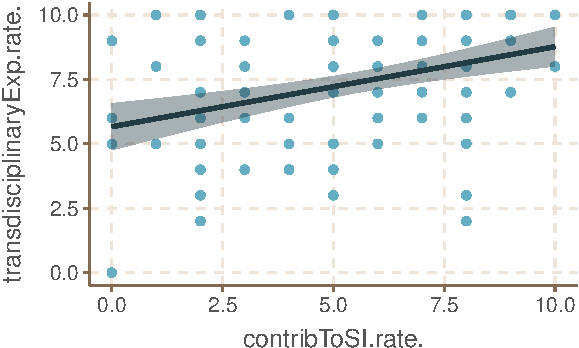
\includegraphics{03_SIVOCS_int-cand_files/figure-latex/td_si_lm-1}

While transdisciplinarity shows some relation to SI, its meaning can be
different among different disciplines. The cluster in the second step
has been divided into \emph{STEM} and \emph{other disciplines} before
examining further.

The examination of the participants from \emph{STEM} disciplines with
high disciplinarity experience included along with \emph{contribution
tho SI} the analysis of the \emph{motivation} for the study (e.g.~either
human condition/welfare was part of the motivation) and which other
societal actors were involved in the project. Finally, because of the
unsatisfactory representation of the female participants in the cluster,
a slight bias toward female participants from STEM fields has been
added. This examination yielded 3 candidates for the interview process
(2m \textbar{} 1f).

Non-STEM fields were also subjected to a similar analysis regarding
\emph{contribution to SI} and different kinds of involvements. A manual
examination was also needed because of the large spectrum of those
disciplines. 19 participants have been selected in this cluster in total
(4f \textbar{} 15m)

\hypertarget{step-3-motivation-to-improve-the-human-conditionwelfare-involvement-of-the-civil-society-civil-soc.s-nature-of-the-involvement}{%
\section{Step 3: Motivation to improve the human condition/welfare,
involvement of the civil society, civil soc.'s nature of the
involvement}\label{step-3-motivation-to-improve-the-human-conditionwelfare-involvement-of-the-civil-society-civil-soc.s-nature-of-the-involvement}}

Variables \emph{motivation to improve the human condition} and
\emph{rate of involvement of the civil soc.} do not necessarily show a
strong correlation (see Figure @ref(fig:wf\_fi\_lm)). However, including
the \emph{nature of involvement} of civil society groups yields
relatively better results (\emph{nature of involvement} collaboration or
cocreation against the other forms of collaboration is described in the
second figure). Therefore, step 3 has focused on the projects with high
motivation to improve human condition and citizen involvement where the
nature of the involvement is either collaboration or co-creation. This
approach yielded 7 participants (1f \textbar{} 6m).

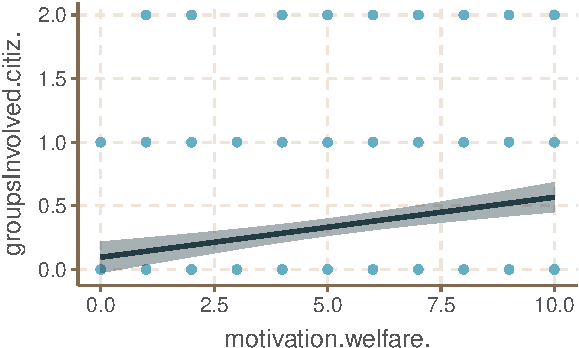
\includegraphics{03_SIVOCS_int-cand_files/figure-latex/wf_gi_lm-1}
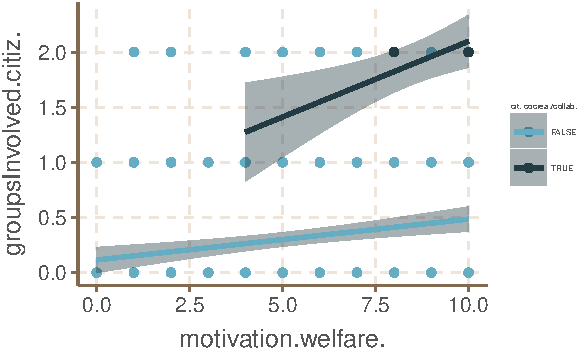
\includegraphics{03_SIVOCS_int-cand_files/figure-latex/wf_gi_lm-2}

\hypertarget{step-4-familiarity-with-si}{%
\section{Step 4: Familiarity with SI}\label{step-4-familiarity-with-si}}

Considering the observations in the study correspond to the projects and
not the researchers themselves, it is fairly possible to overlook
researchers with SI experience and SI-related (SNF-funded) projects just
because the specific project was not necessarily an SI-related project.
In order to combat this issue step 4 started with the consideration of
high values (again between 3rd quantile and max values) of
\emph{familiarity with SI}.

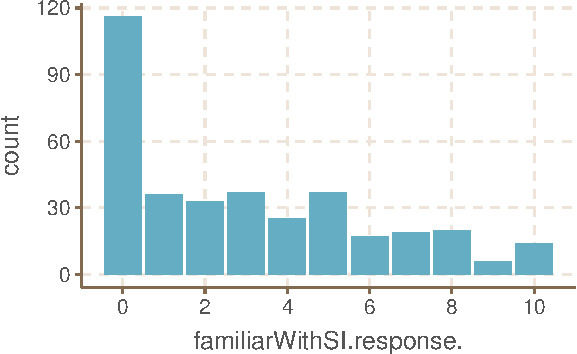
\includegraphics{03_SIVOCS_int-cand_files/figure-latex/step4-1} This
relatively small cluster has been also analyzed manually with the
consideration of answers to open and meta-questions like
\emph{feedback}, \emph{title of the project} etc., some of the
participants were specially selected for their critical feedback on the
nature of the study. This process added 8 more participants to the list.

\hypertarget{final}{%
\chapter{Final}\label{final}}

After a manual elimination, from the 71 selected projects in total 16
relatively less related projects are eliminated, \textbf{leaving 55
participants in total} (14f \textbar{} 41 \textasciitilde{} 25\%, see
Figure @ref(fig:gender)).

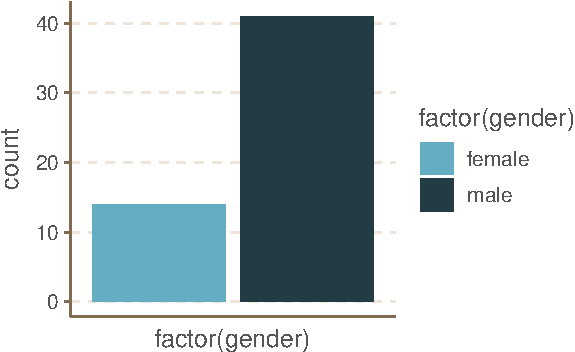
\includegraphics{03_SIVOCS_int-cand_files/figure-latex/gender-1}

Also, the distribution of the sci. disciplines in the final sample is as
follows:

\begin{longtable}[]{@{}lr@{}}
\toprule()
Var1 & Freq \\
\midrule()
\endhead
Architecture and Social urban science & 1 \\
Arts & 1 \\
Biophysics & 1 \\
Economics & 3 \\
Education and learning sciences, subject-specific education & 5 \\
Ethnology & 2 \\
Experimental Microbiology & 1 \\
General history (without pre-and early history) & 1 \\
German and English languages and literature & 1 \\
Information Technology & 2 \\
Inorganic Chemistry & 2 \\
Legal sciences & 1 \\
Molecular Biology & 2 \\
Music, Theatre & 1 \\
Neurophysiology and Brain Research & 3 \\
Other languages and literature & 2 \\
Philosophy & 1 \\
Political science & 2 \\
Psychology & 4 \\
Religious studies, Theology & 2 \\
Romance languages and literature & 1 \\
Science of management & 2 \\
Social geography and ecology & 2 \\
Social work & 3 \\
Sociology & 1 \\
Swiss history & 4 \\
Technical Physics & 1 \\
Visual arts and Art history & 2 \\
Zoology & 1 \\
\bottomrule()
\end{longtable}

\bibliography{skeleton.bib}



\end{document}
